\chapter{Learning Prob. Submodular Models} \label{ch:genes}

\section{Introduction}

\section{Sampling for Approximate Maximum Likelihood Learning}

\section{Application: Modeling Mutually Exclusive Cancer Genes}
\subsection{Previous Approaches}
\subsection{Experimental Setup}

\section{Sythetic Data}
\subsection{Real Cancer Data}

\subsection{AML data}

\begin{figure}[htb]
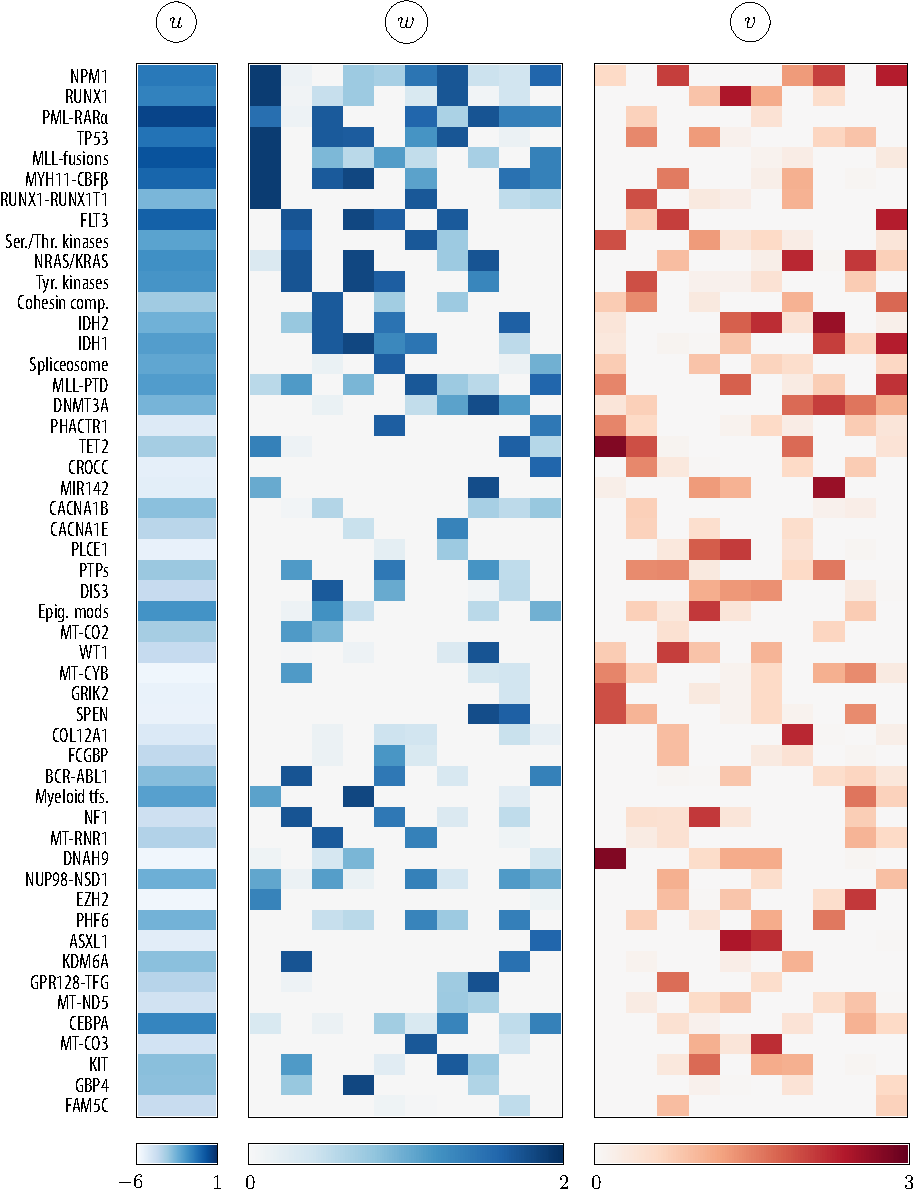
\includegraphics[width=\textwidth]{figures/genes/mat_aml.pdf}\\[2em]
\caption{Test}
\end{figure}

\begin{figure}[htb]
\centering
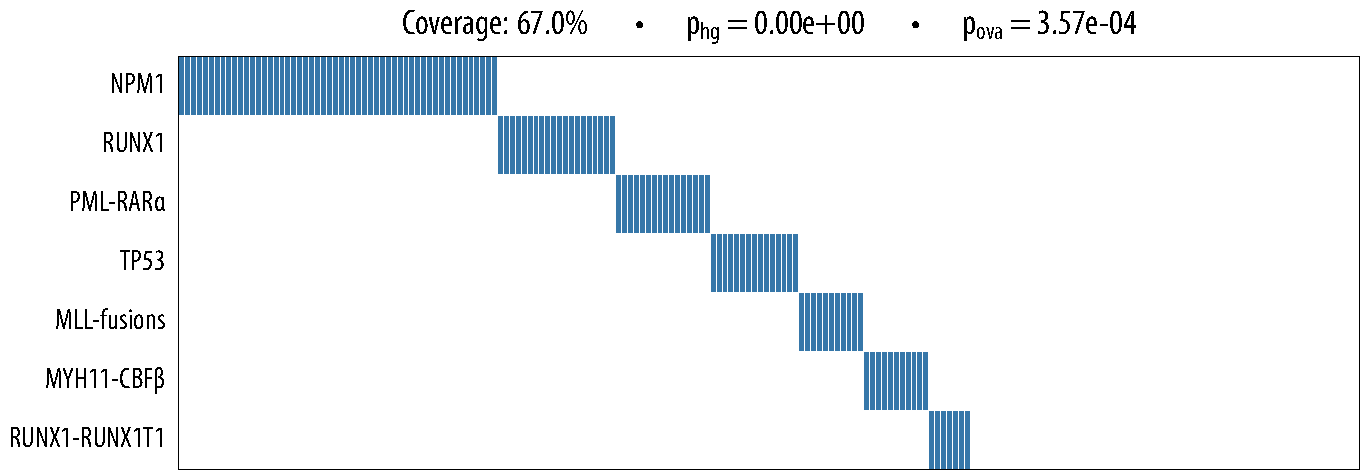
\includegraphics[width=\textwidth]{figures/genes/aml_1.pdf}\\[2em]
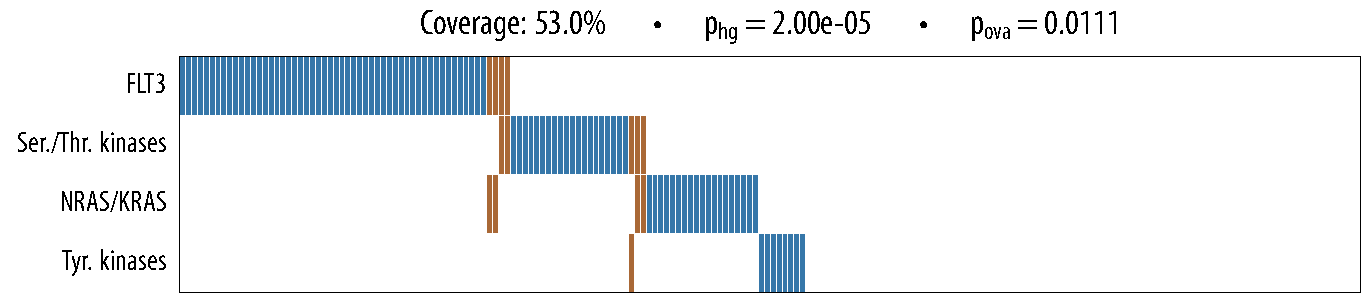
\includegraphics[width=\textwidth]{figures/genes/aml_2.pdf}\\[2em]
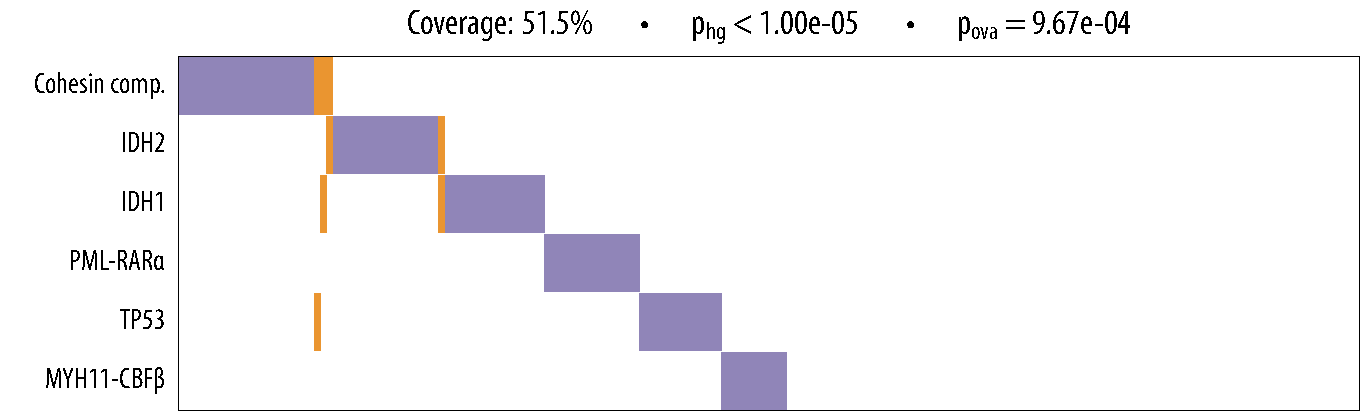
\includegraphics[width=\textwidth]{figures/genes/aml_3.pdf}\\[2em]
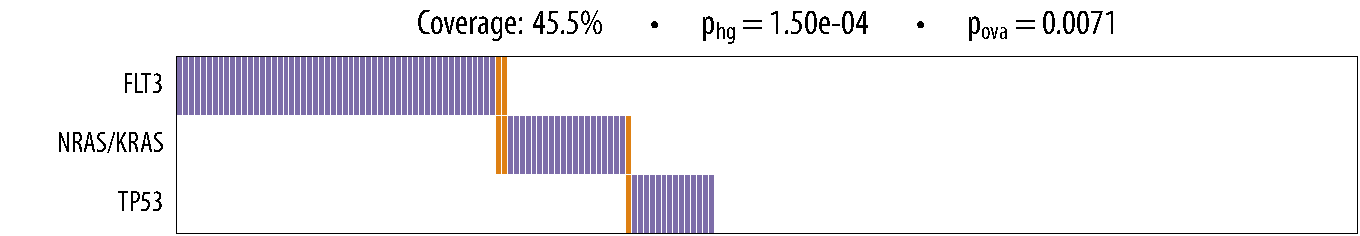
\includegraphics[width=\textwidth]{figures/genes/aml_4.pdf}\\[2em]
\caption{Test}
\end{figure}

\begin{figure}[htb]
\centering
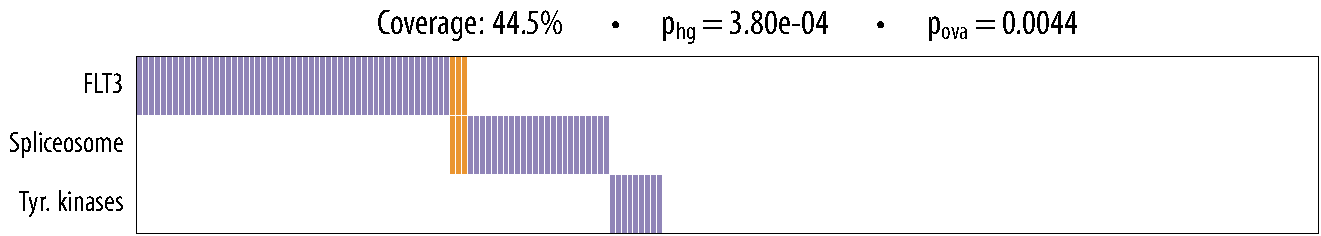
\includegraphics[width=\textwidth]{figures/genes/aml_5.pdf}\\[2em]
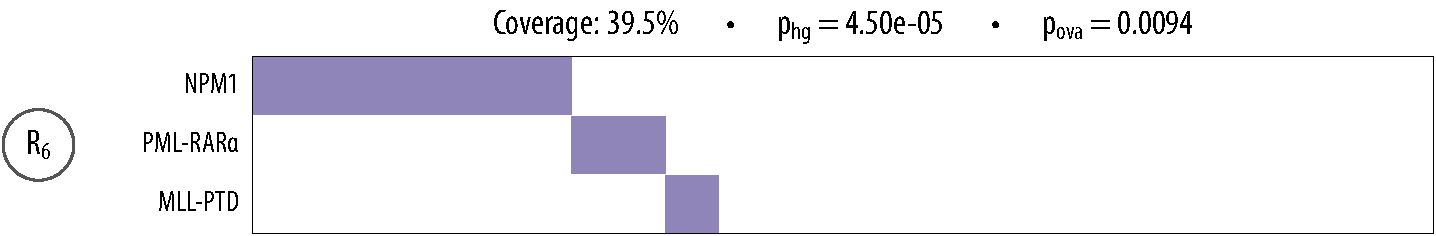
\includegraphics[width=\textwidth]{figures/genes/aml_6.pdf}\\[2em]
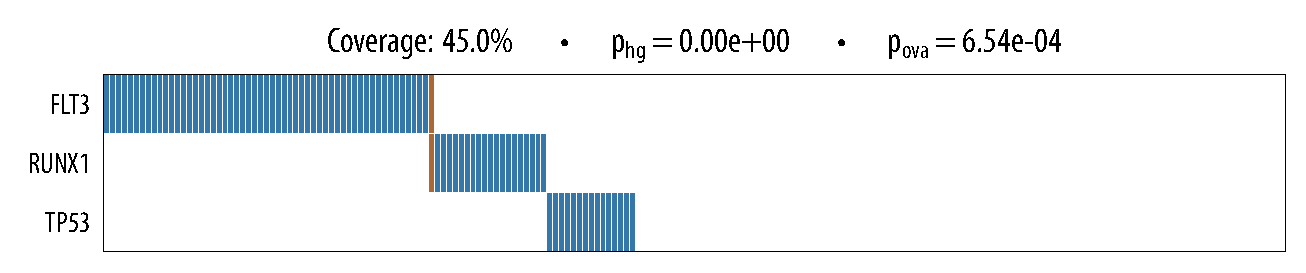
\includegraphics[width=\textwidth]{figures/genes/aml_7.pdf}\\[2em]
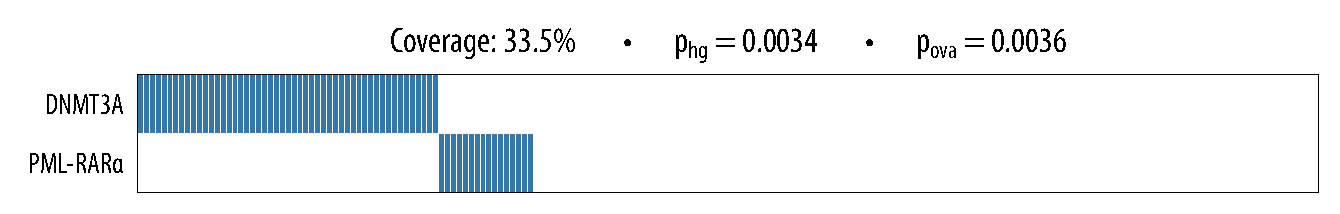
\includegraphics[width=\textwidth]{figures/genes/aml_8.pdf}\\[2em]
\caption{Test}
\end{figure}

\begin{figure}[htb]
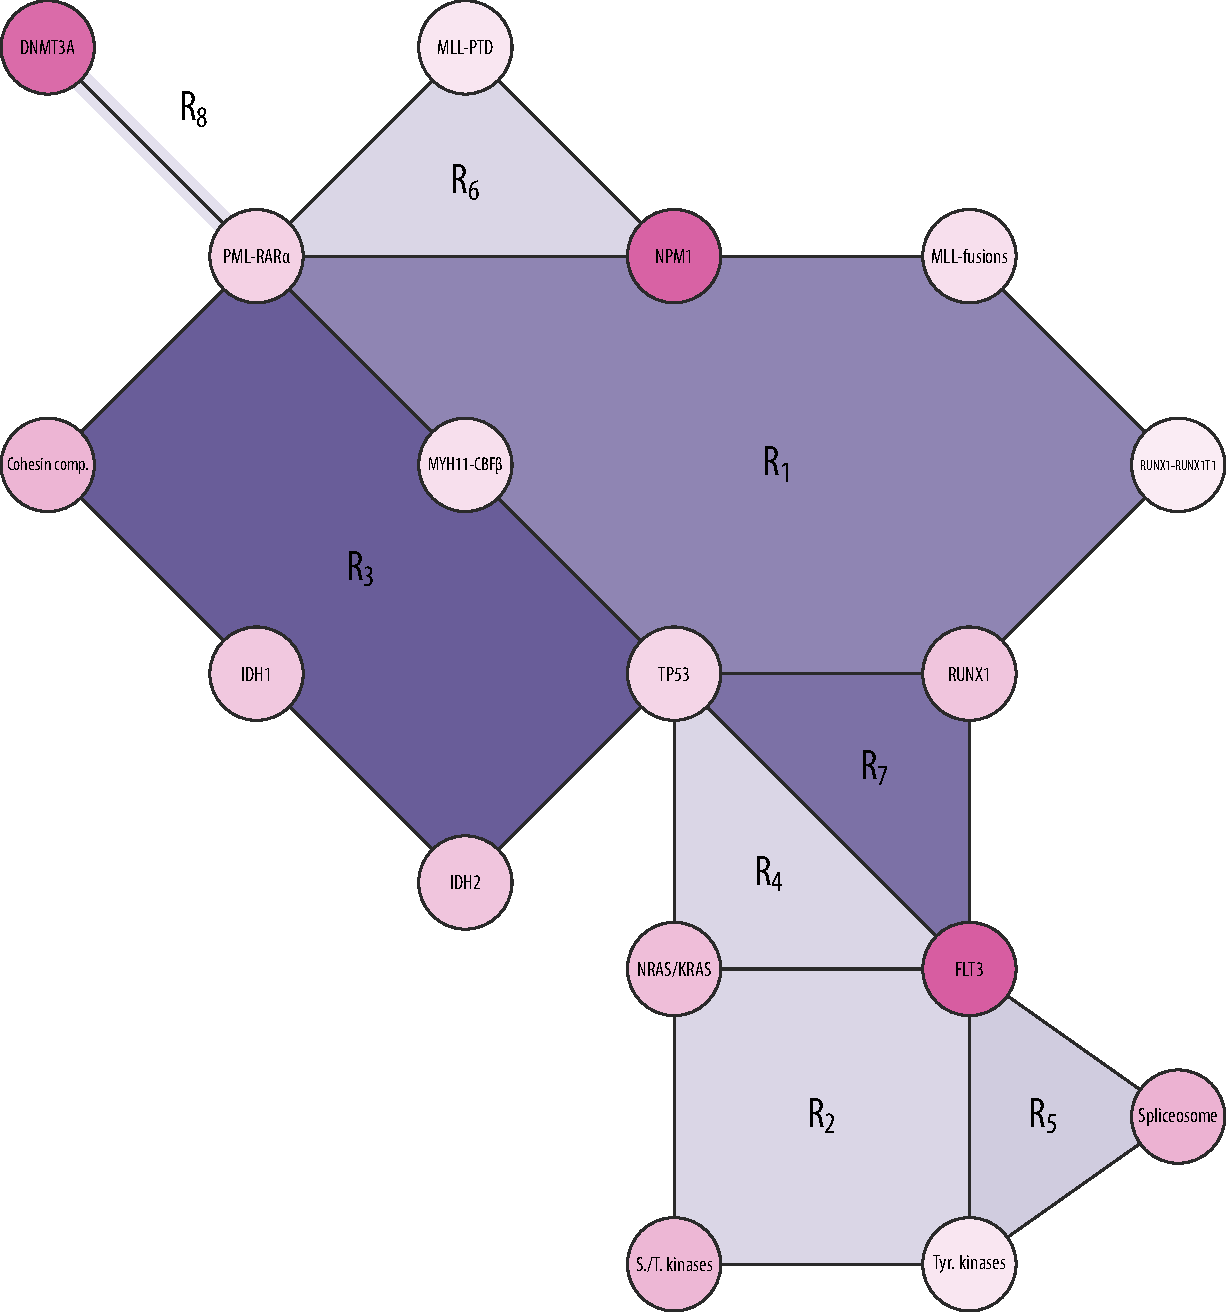
\includegraphics[width=\textwidth]{figures/genes/graph_aml.pdf}\\[2em]
\caption{AML repulsive graph}
\end{figure}

\begin{figure}[htb]
\centering
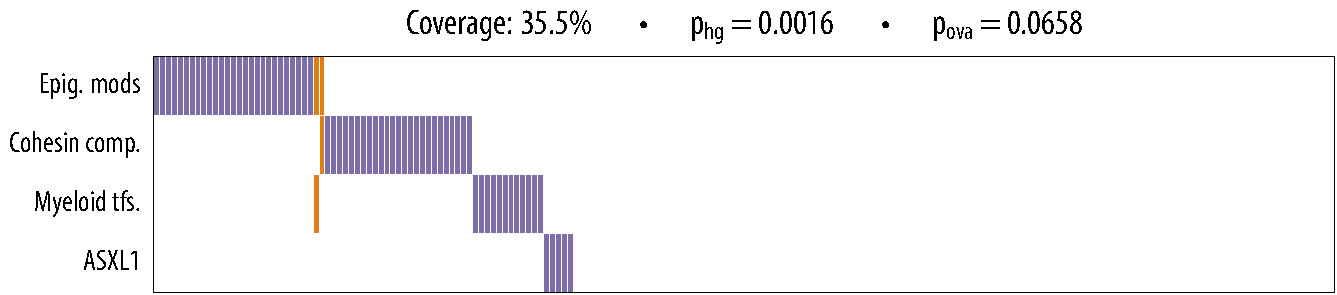
\includegraphics[width=\textwidth]{figures/genes/aml_comet1.pdf}\\[2em]
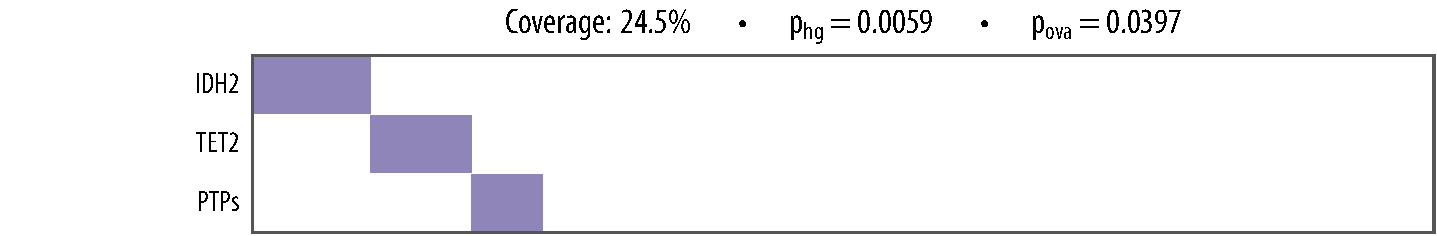
\includegraphics[width=\textwidth]{figures/genes/aml_comet2.pdf}\\[2em]
\caption{CoMEt extra groups (probably appendix)}
\end{figure}

\begin{figure}[htb]
\centering
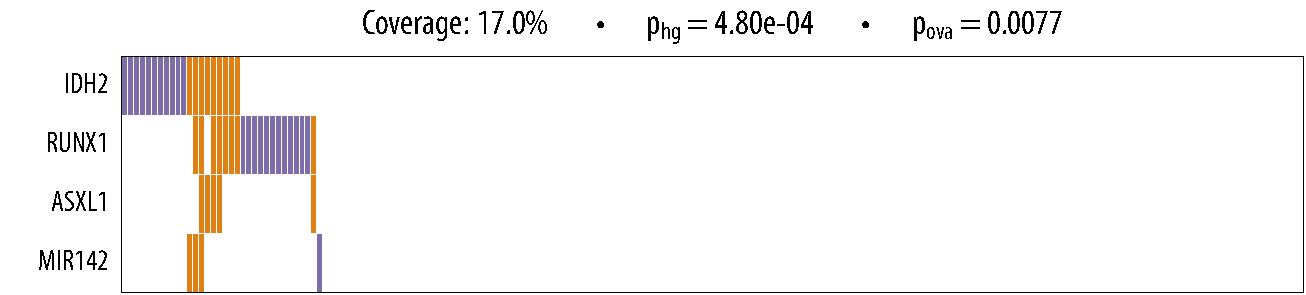
\includegraphics[width=\textwidth]{figures/genes/aml_2_a.pdf}\\[2em]
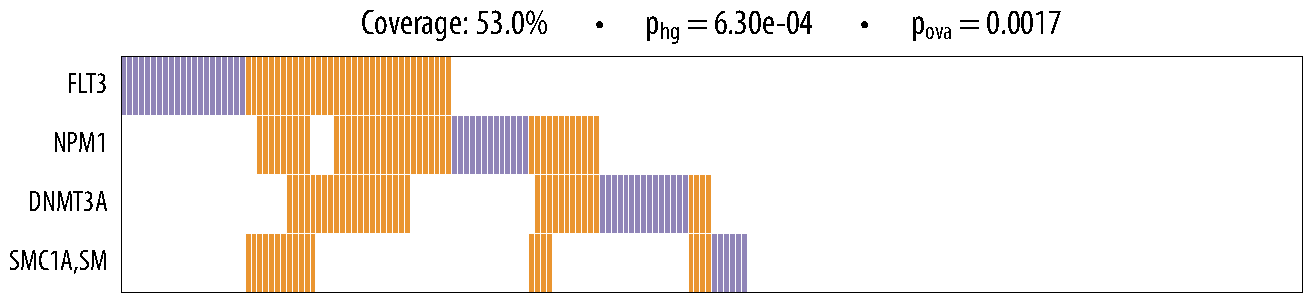
\includegraphics[width=\textwidth]{figures/genes/aml_1_a.pdf}\\[2em]
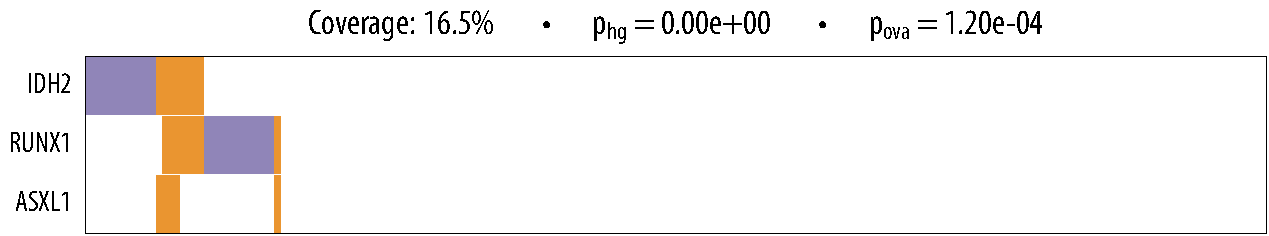
\includegraphics[width=\textwidth]{figures/genes/aml_3_a.pdf}\\[2em]
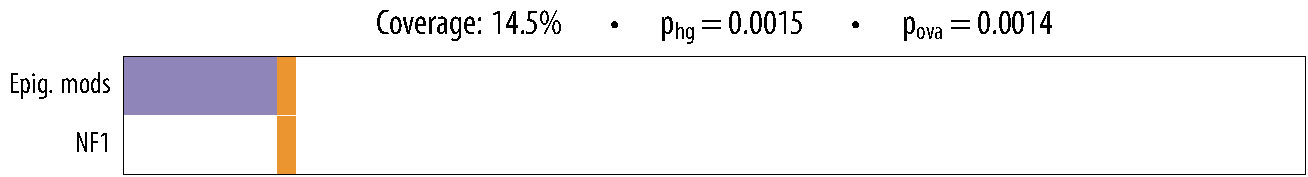
\includegraphics[width=\textwidth]{figures/genes/aml_5_a.pdf}\\[2em]
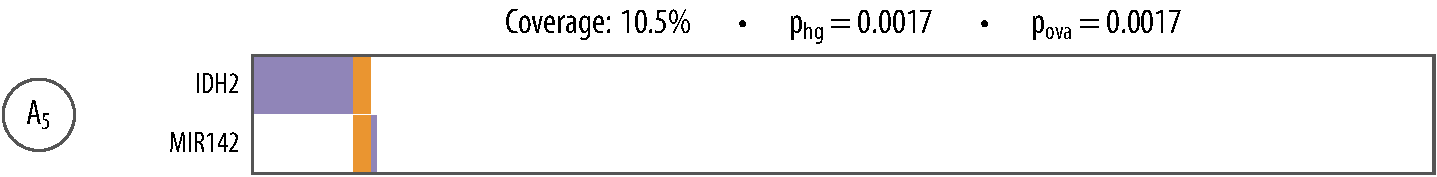
\includegraphics[width=\textwidth]{figures/genes/aml_4_a.pdf}\\[2em]
\caption{Test}
\end{figure}

\subsection{BRCA data}
\begin{figure}[htb]
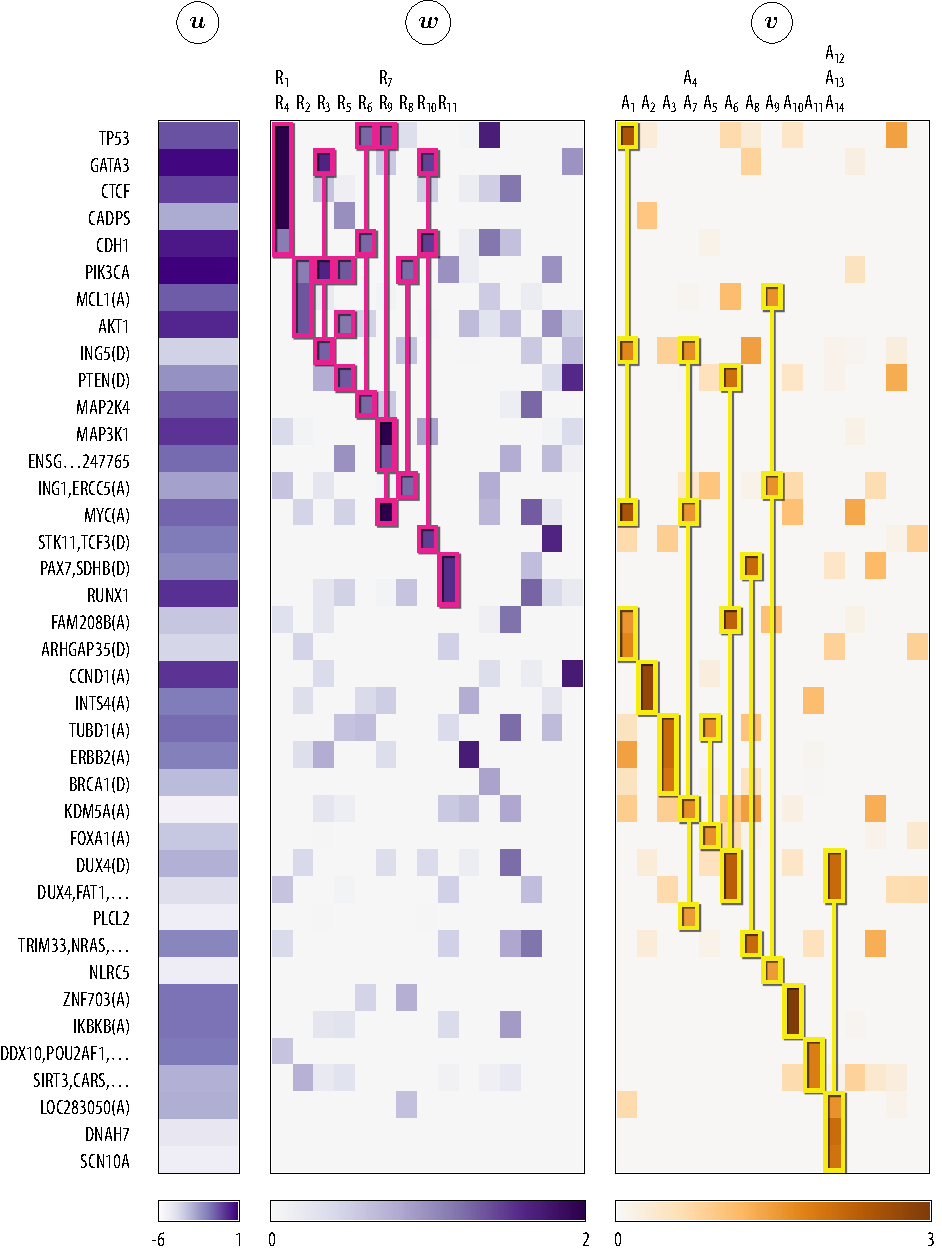
\includegraphics[width=\textwidth]{figures/genes/mat_brca.pdf}\\[2em]
\caption{Test}
\end{figure}

\begin{figure}[htb]
\centering
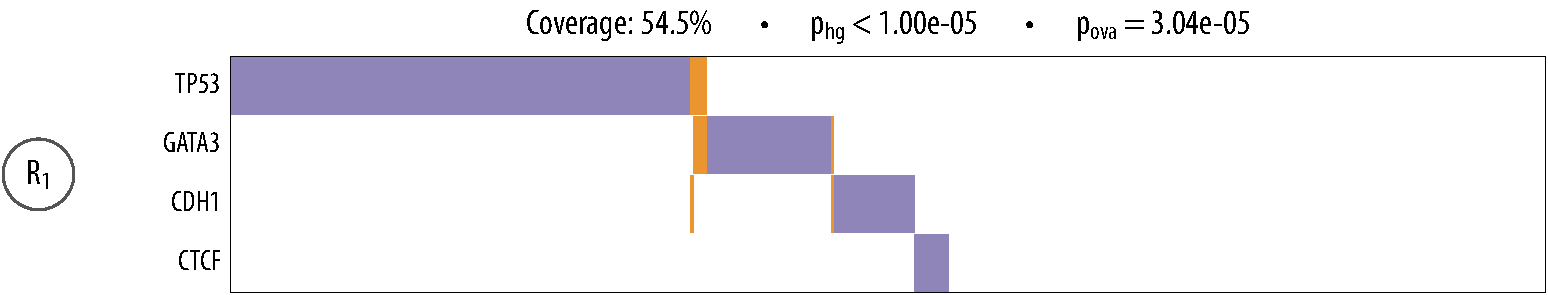
\includegraphics[width=\textwidth]{figures/genes/brca_1.pdf}\\[2em]
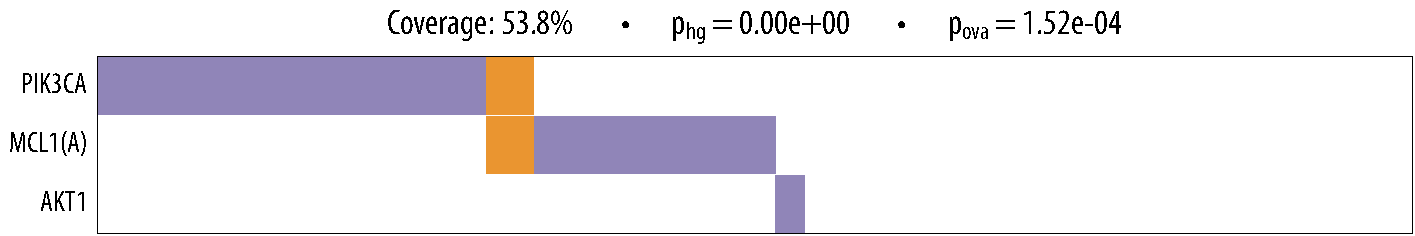
\includegraphics[width=\textwidth]{figures/genes/brca_6.pdf}\\[2em]
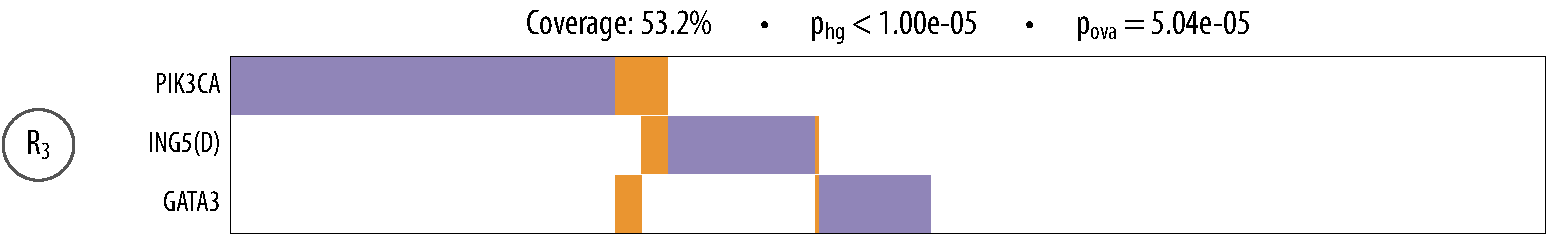
\includegraphics[width=\textwidth]{figures/genes/brca_8.pdf}\\[2em]
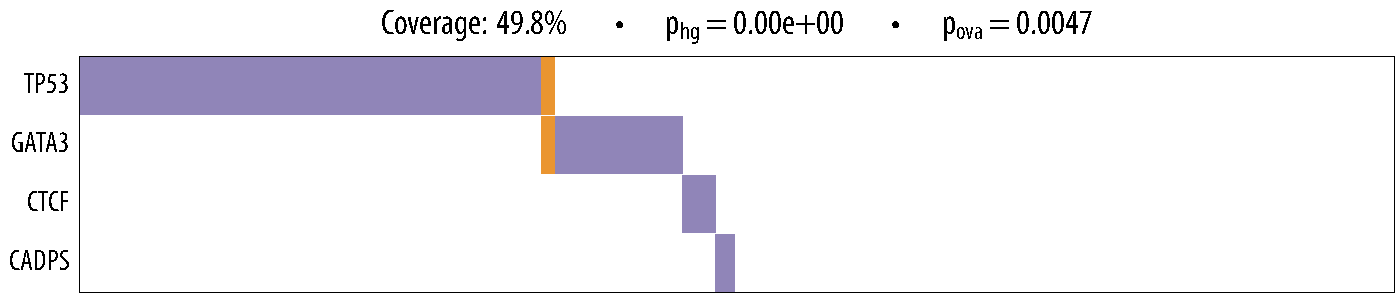
\includegraphics[width=\textwidth]{figures/genes/brca_2.pdf}\\[2em]
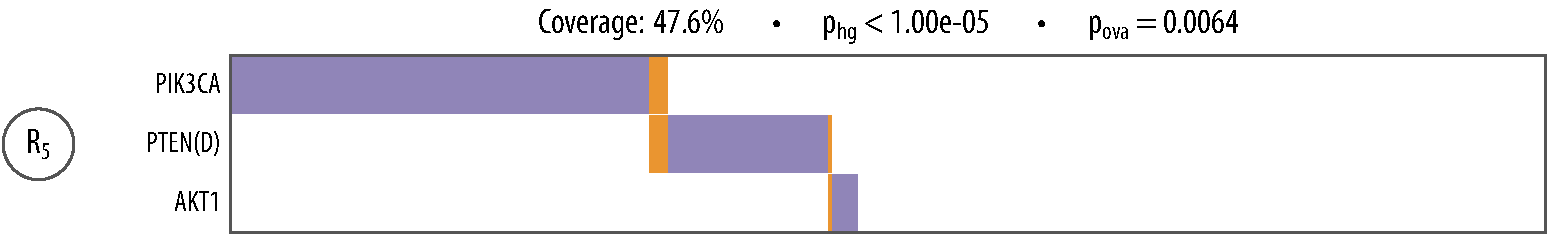
\includegraphics[width=\textwidth]{figures/genes/brca_5.pdf}\\[2em]
\caption{BRCA repulsive (I)}
\end{figure}

\begin{figure}[htb]
\centering
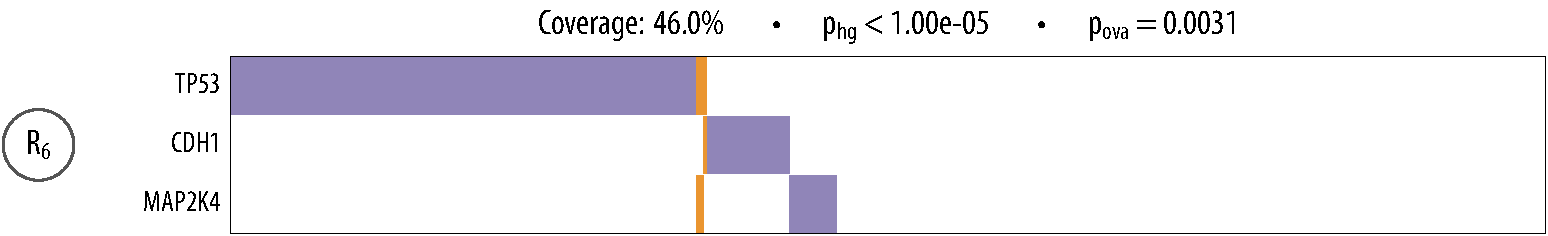
\includegraphics[width=\textwidth]{figures/genes/brca_4.pdf}\\[2em]
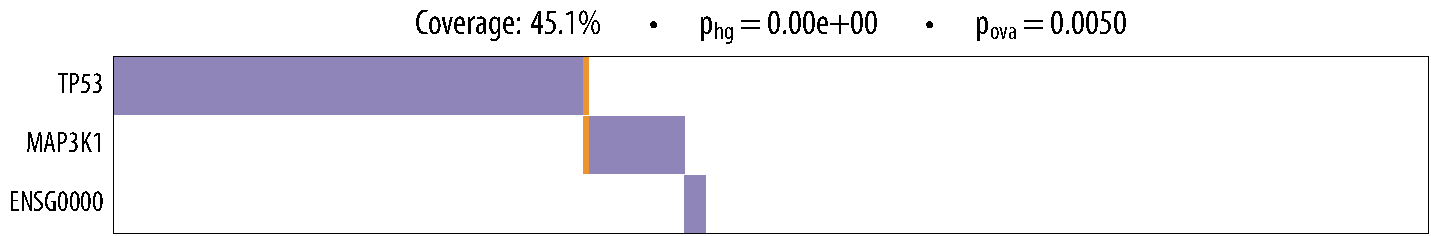
\includegraphics[width=\textwidth]{figures/genes/brca_3.pdf}\\[2em]
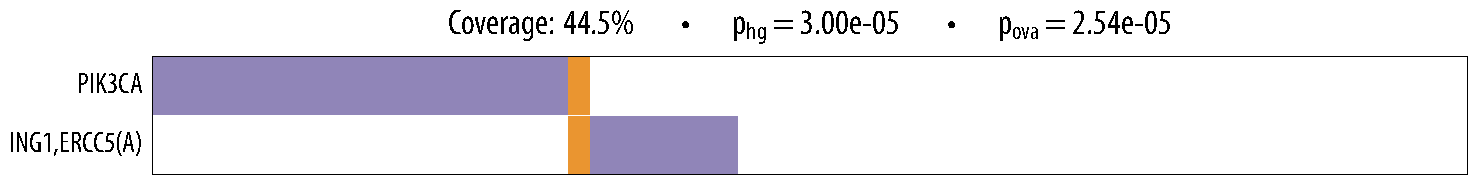
\includegraphics[width=\textwidth]{figures/genes/brca_11.pdf}\\[2em]
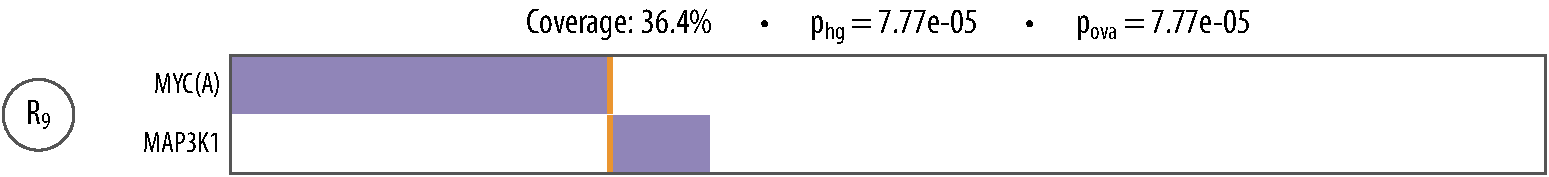
\includegraphics[width=\textwidth]{figures/genes/brca_10.pdf}\\[2em]
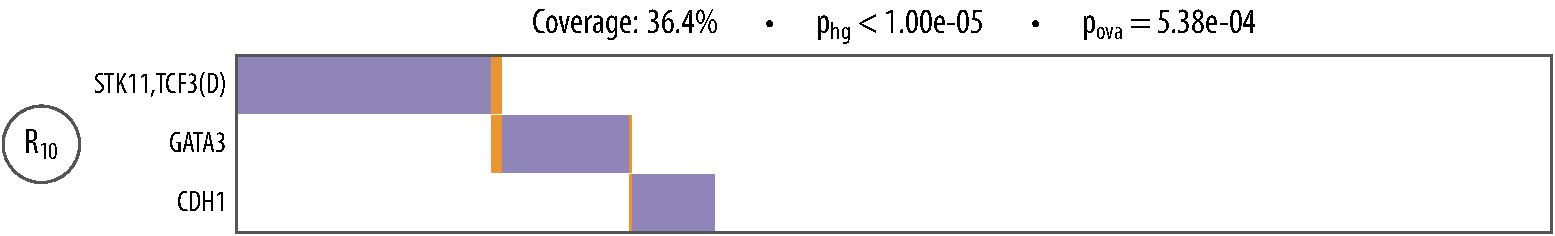
\includegraphics[width=\textwidth]{figures/genes/brca_7.pdf}\\[2em]
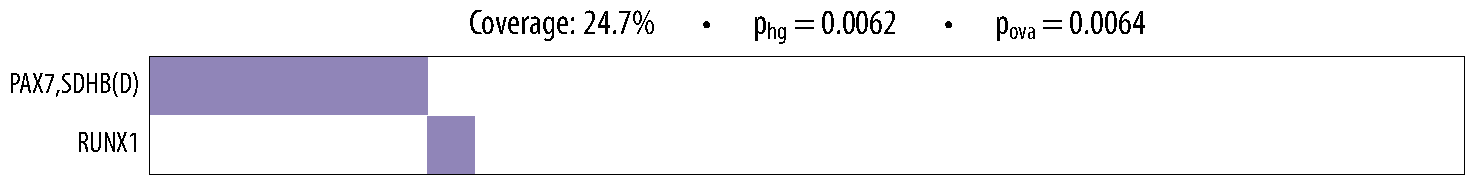
\includegraphics[width=\textwidth]{figures/genes/brca_9.pdf}\\[2em]
\caption{BRCA repulsive (II)}
\end{figure}

\begin{figure}[htb]
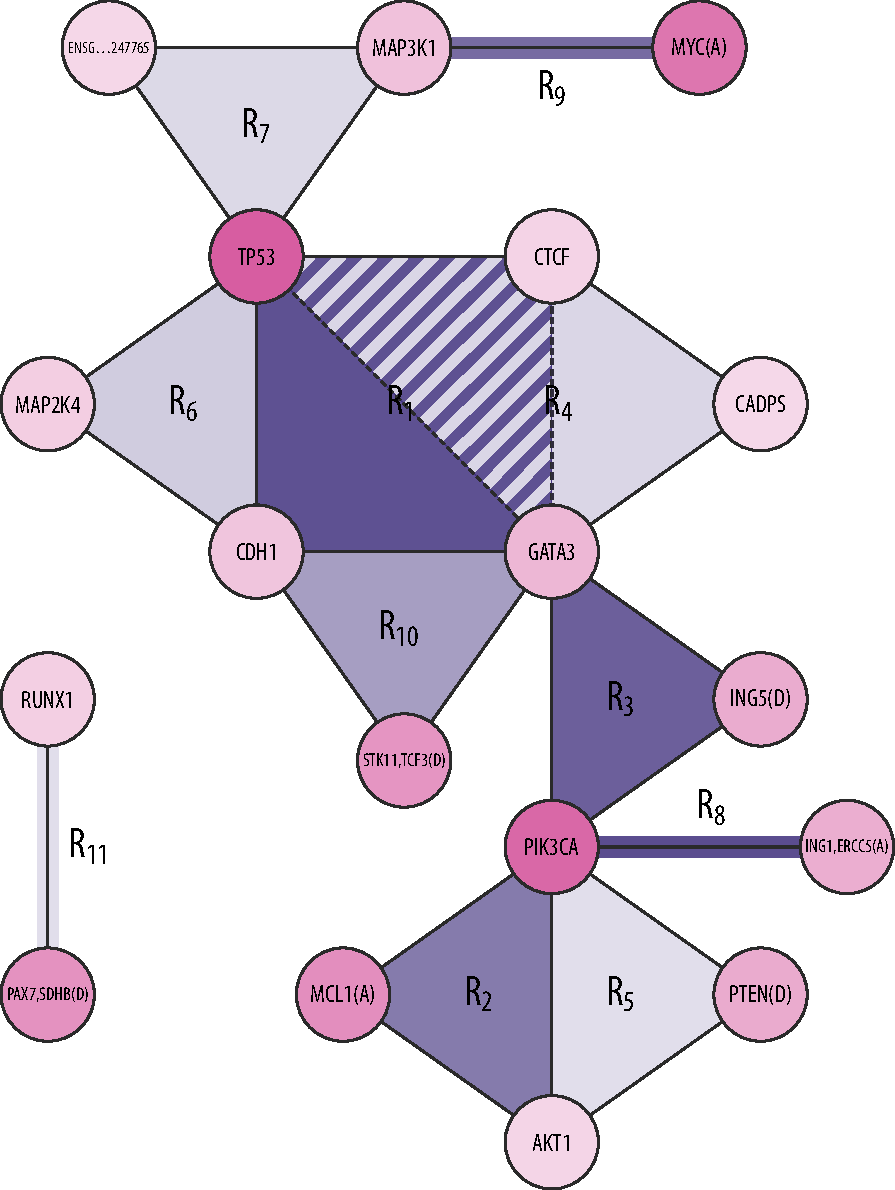
\includegraphics[width=\textwidth]{figures/genes/graph_brca.pdf}\\[2em]
\caption{BRCA repulsive graph}
\end{figure}

\begin{figure}[htb]
\centering
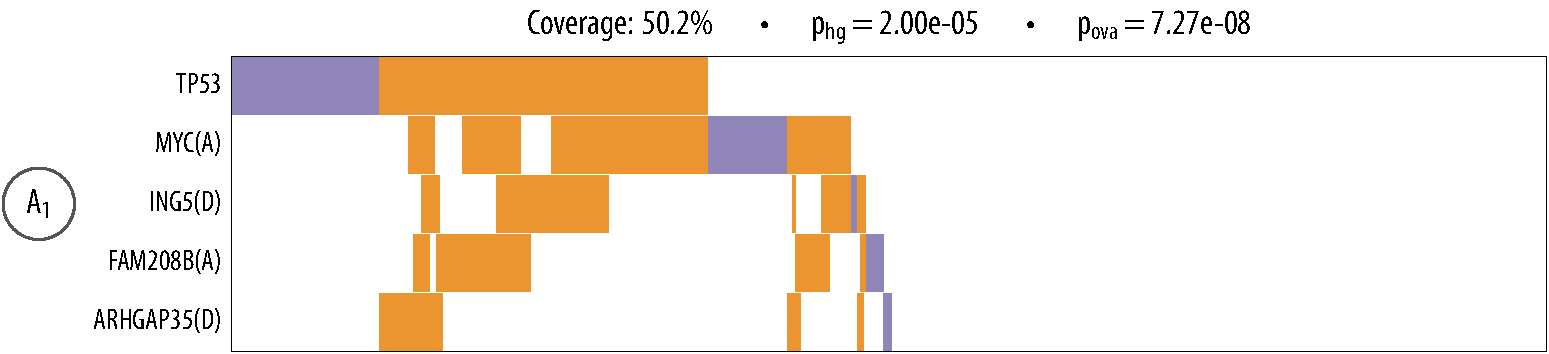
\includegraphics[width=\textwidth]{figures/genes/brca_1_a.pdf}\\[2em]
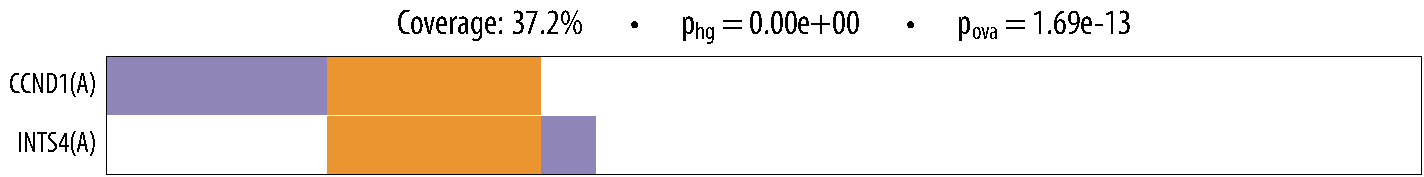
\includegraphics[width=\textwidth]{figures/genes/brca_11_a.pdf}\\[2em]
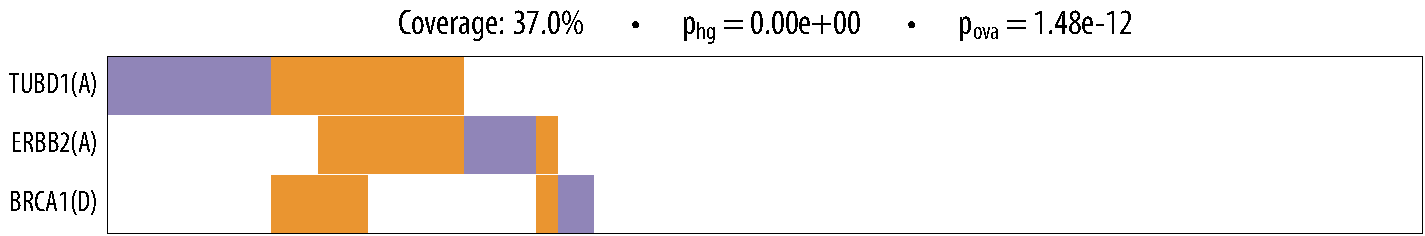
\includegraphics[width=\textwidth]{figures/genes/brca_7_a.pdf}\\[2em]
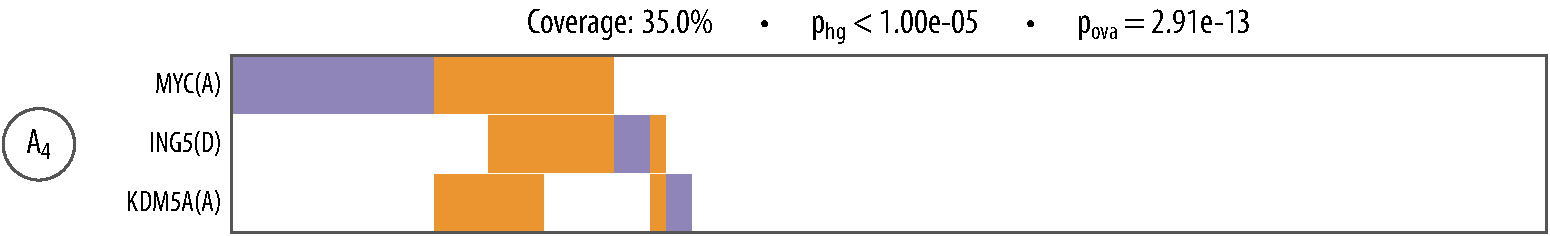
\includegraphics[width=\textwidth]{figures/genes/brca_8_a.pdf}\\[2em]
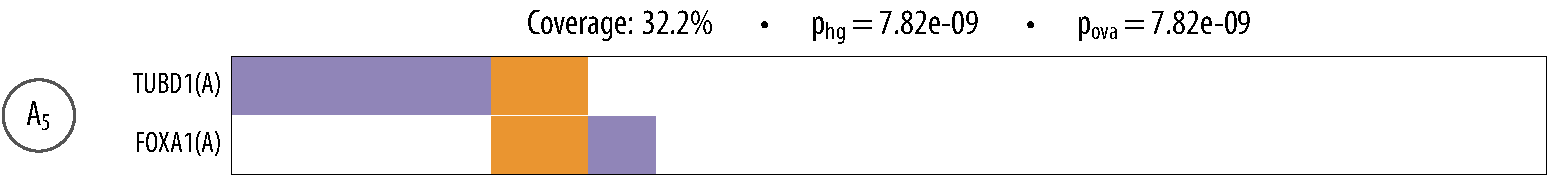
\includegraphics[width=\textwidth]{figures/genes/brca_14_a.pdf}\\[2em]
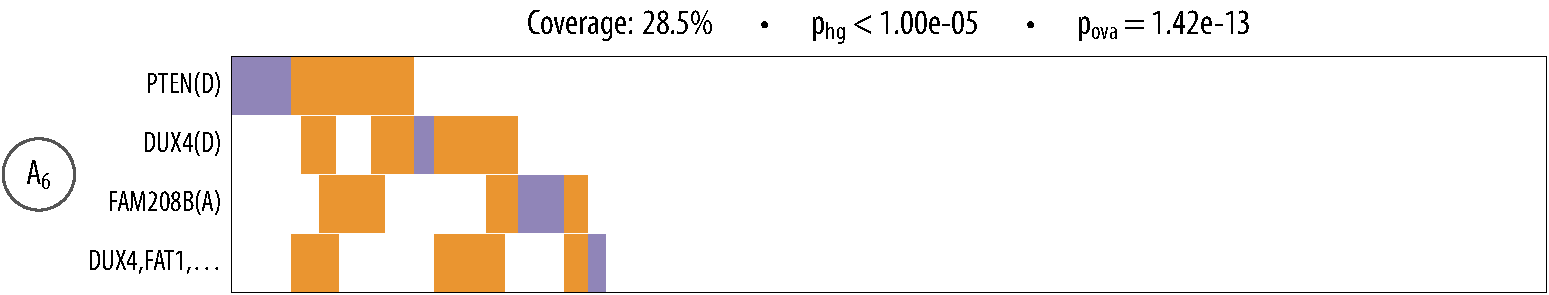
\includegraphics[width=\textwidth]{figures/genes/brca_4_a.pdf}\\[2em]
\caption{BRCA attractive}
\end{figure}

\begin{figure}[htb]
\centering
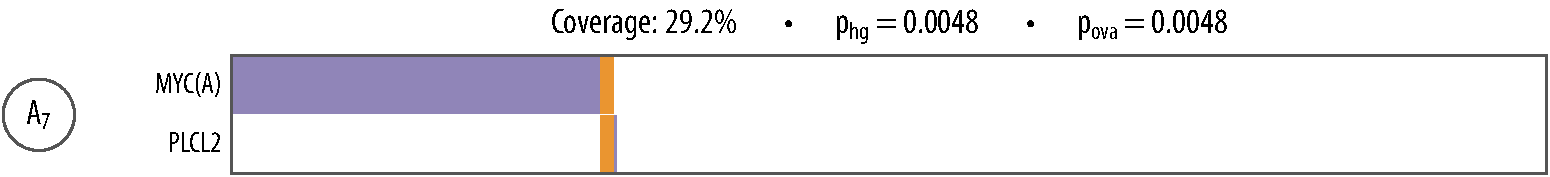
\includegraphics[width=\textwidth]{figures/genes/brca_9_a.pdf}\\[2em]
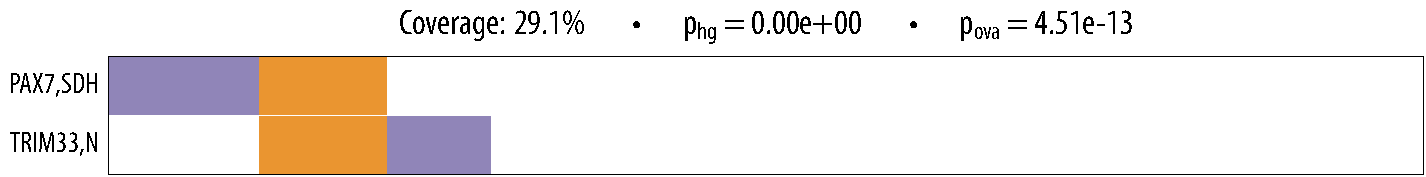
\includegraphics[width=\textwidth]{figures/genes/brca_13_a.pdf}\\[2em]
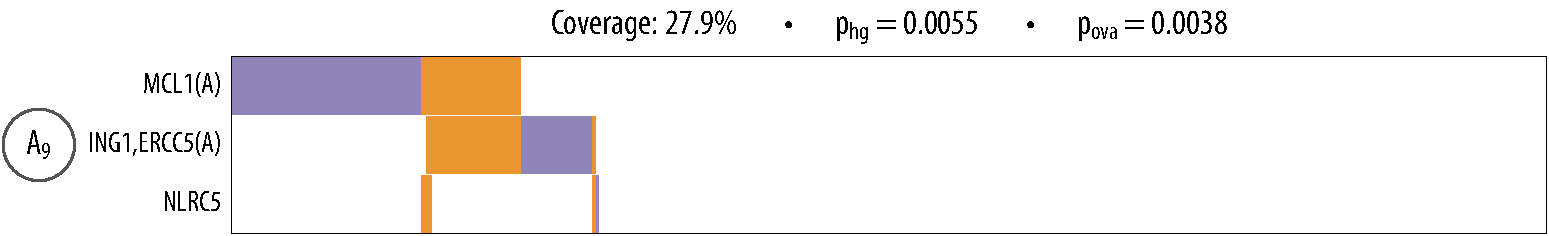
\includegraphics[width=\textwidth]{figures/genes/brca_5_a.pdf}\\[2em]
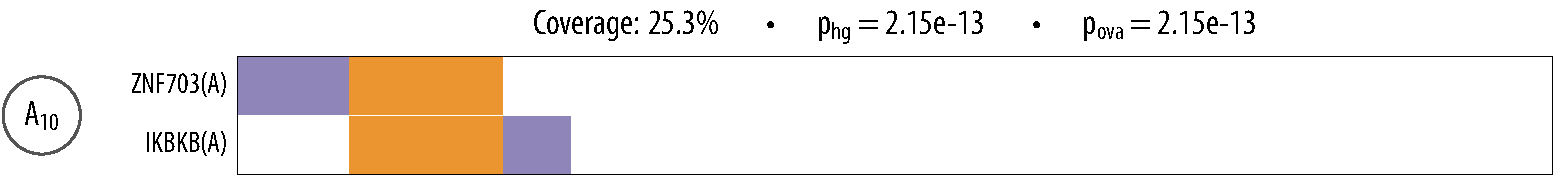
\includegraphics[width=\textwidth]{figures/genes/brca_10_a.pdf}\\[2em]
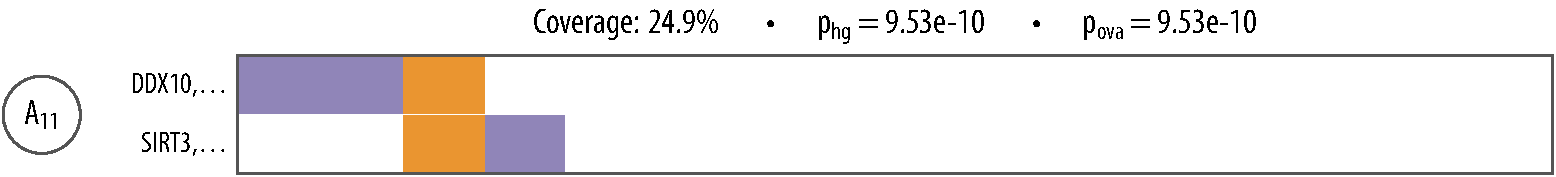
\includegraphics[width=\textwidth]{figures/genes/brca_12_a.pdf}\\[2em]
\caption{BRCA attractive (appendix I)}
\end{figure}

\begin{figure}[htb]
\centering
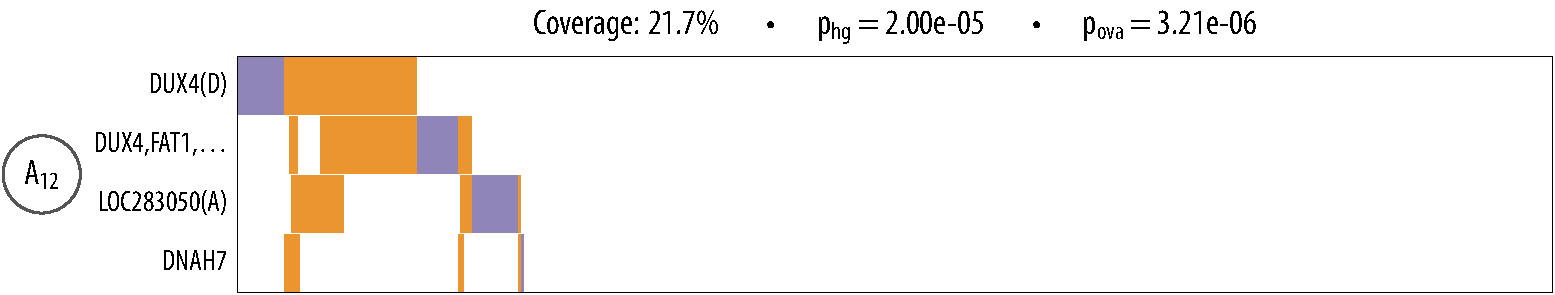
\includegraphics[width=\textwidth]{figures/genes/brca_3_a.pdf}\\[2em]
%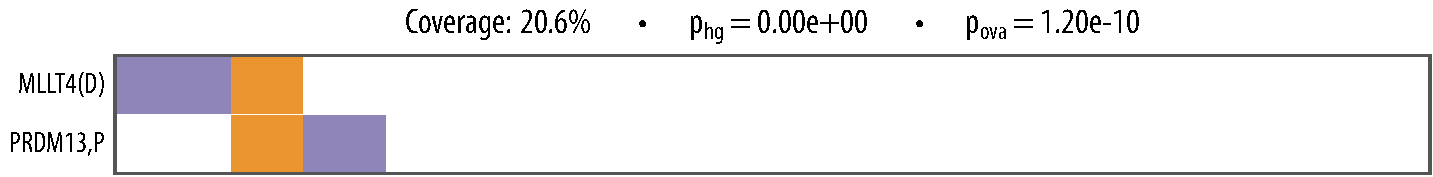
\includegraphics[width=\textwidth]{figures/genes/brca_15_a.pdf}\\[2em]
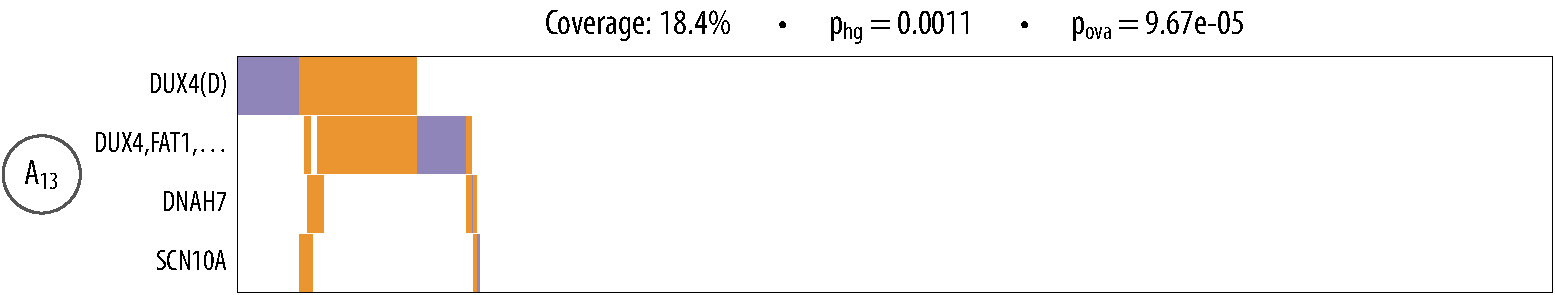
\includegraphics[width=\textwidth]{figures/genes/brca_2_a.pdf}\\[2em]
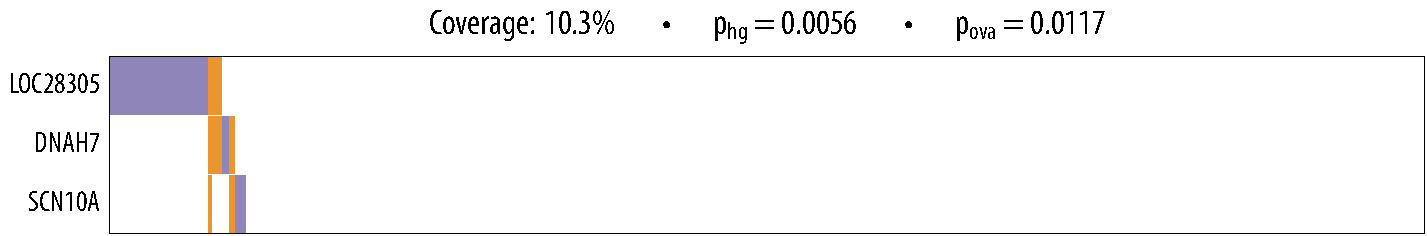
\includegraphics[width=\textwidth]{figures/genes/brca_6_a.pdf}\\[2em]
\caption{BRCA attractive (appendix II)}
\end{figure}

\section{Conclusion}